\chapter{Systembeskrivelse}
\section{Systemoversigt}

	\begin{figure}[h!]
		\centering
		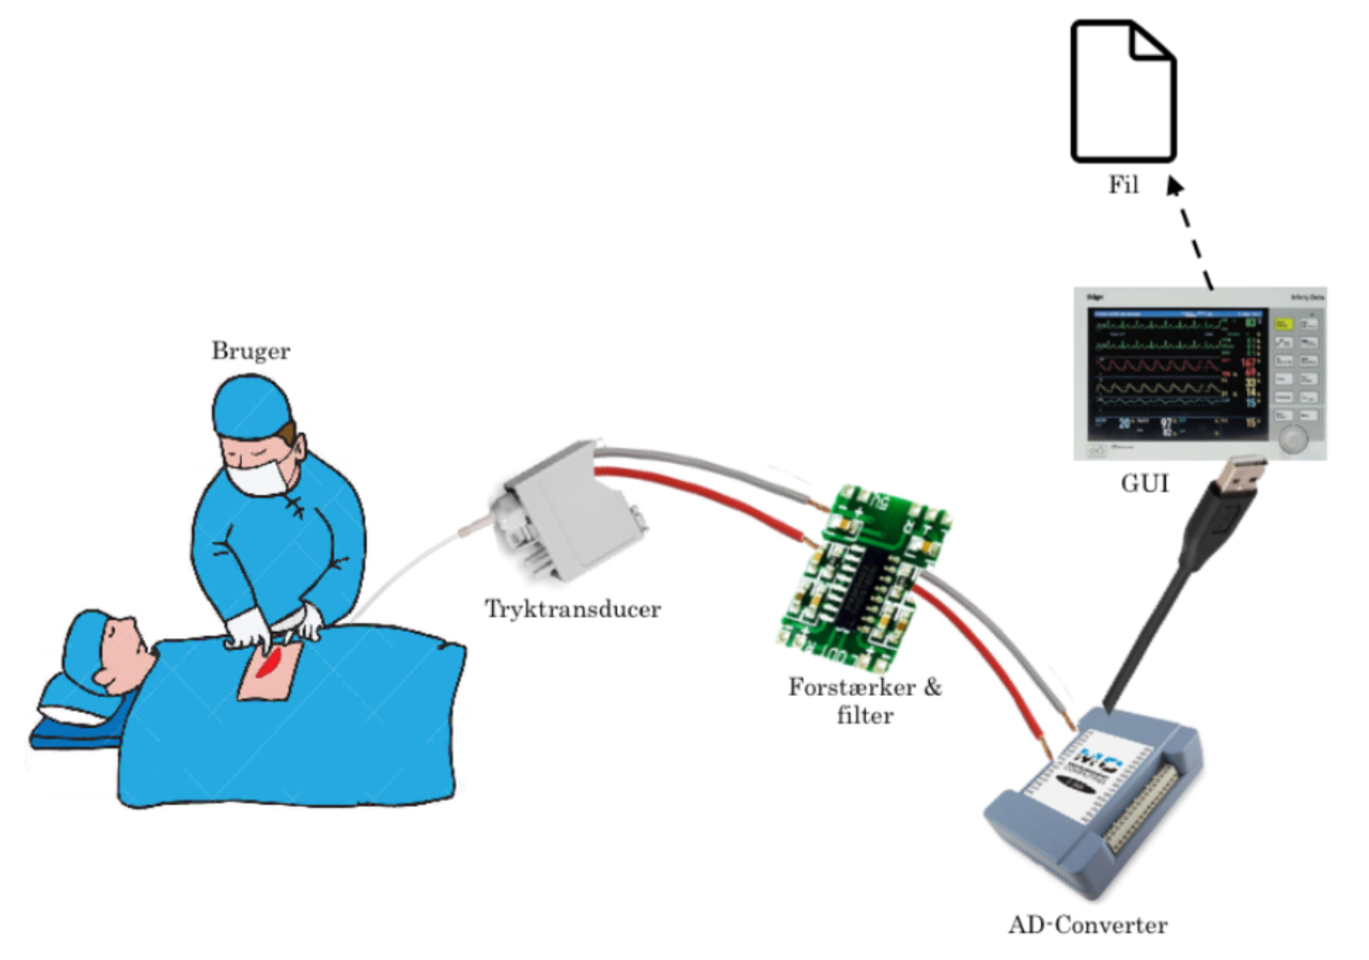
\includegraphics[width=0.55\linewidth]{Systembeskrivelse/Systemoversigt}
		\caption{Systemoversigt}
		\label{fig:Systemoversigt}
	\end{figure}
\vspace{1 cm}

\section{Systembeskrivelse}
På figur \ref{fig:Systemoversigt} ses en systemoversigt over et blodtrykmålesystem, der har til formål at kunne måle og vise en patients blodtryk og puls på en brugergrænseflade. 

Systemet består af:

\begin{itemize}
	\item Tryktransducer
	\item Forstærker
	\item Subtraktor
	\item Anti-aliaseringsfilter
	\item AD-Converter (NI DAQ 6009 USB)
	\item Computer
	\item Bluetooth højtaler
	\item Skærm
	\item Brugergrænseflade	
\end{itemize}

Brugergrænsefladen er bygget op som et Graphical User Interface (GUI) hvorpå det målte blodtryk visualiseres kontinuert i form af en graf. Det systoliske-, diastoliske-, median blodtryk og puls vises i form af tal. Brugergrænsefladen består af knapper, der har forskellige funktioner. For nærmere beskrivelse af brugergrænsefladens funktioner henvises der til dokumentet kravsspecifikation. \clearpage

\subsection{Alarmer}
Systemet skal i henhold til standard 60601-1-8 vedrørende alarmering kunne alarmere ved eventuelle fejl eller ændringer. I forhold til brugssituationen af blodtrykmålesystemet vurderes det at systemet skal kunne alarmere ved følgende:

\begin{enumerate}[1.]
	\item Fejl i nulpunktsjustering
	\item Tid til kalibrering
	\item Fald eller stigning i blodtryk uden for de justérbare grænseværdier
	\item Fald eller stigning i puls uden for de justérbare grænseværdier
	\item Fejl i gem data 
\end{enumerate}

Alarmerne prioriteres efter hvorvidt de vurderes til at være i kategorien \textit{high priority}, \textit{medium priority} eller \textit{low priority}. Alarmerne alarmerer enten visuelt, auditivt eller begge dele alt efter, hvor højt de er prioriteret. For krav til alarmerne henvises til dokumentet kravspecifikation afsnit 1.12 og dokumentet standard 60601-1-8. 

\clearpage 